% \section{WAN Bandwidth Characteristics}

% \autoref{fig:aws-bandwidth} shows the available bandwidth between Amazon EC2
% servers (Tokyo, Ireland, N. Virginia, N. California) in our day-long
% measurements. Most inter-continental links (between Ireland and all others,
% between Tokyo and N. Virginia) have limited bandwidth (\textasciitilde
% \SI{50}{Mbps}). Other pairs exhibit large variations from \SI{10}{Mbps} up to
% \SI{150}{Mbps}.

% \begin{figure}
%   \centering
%   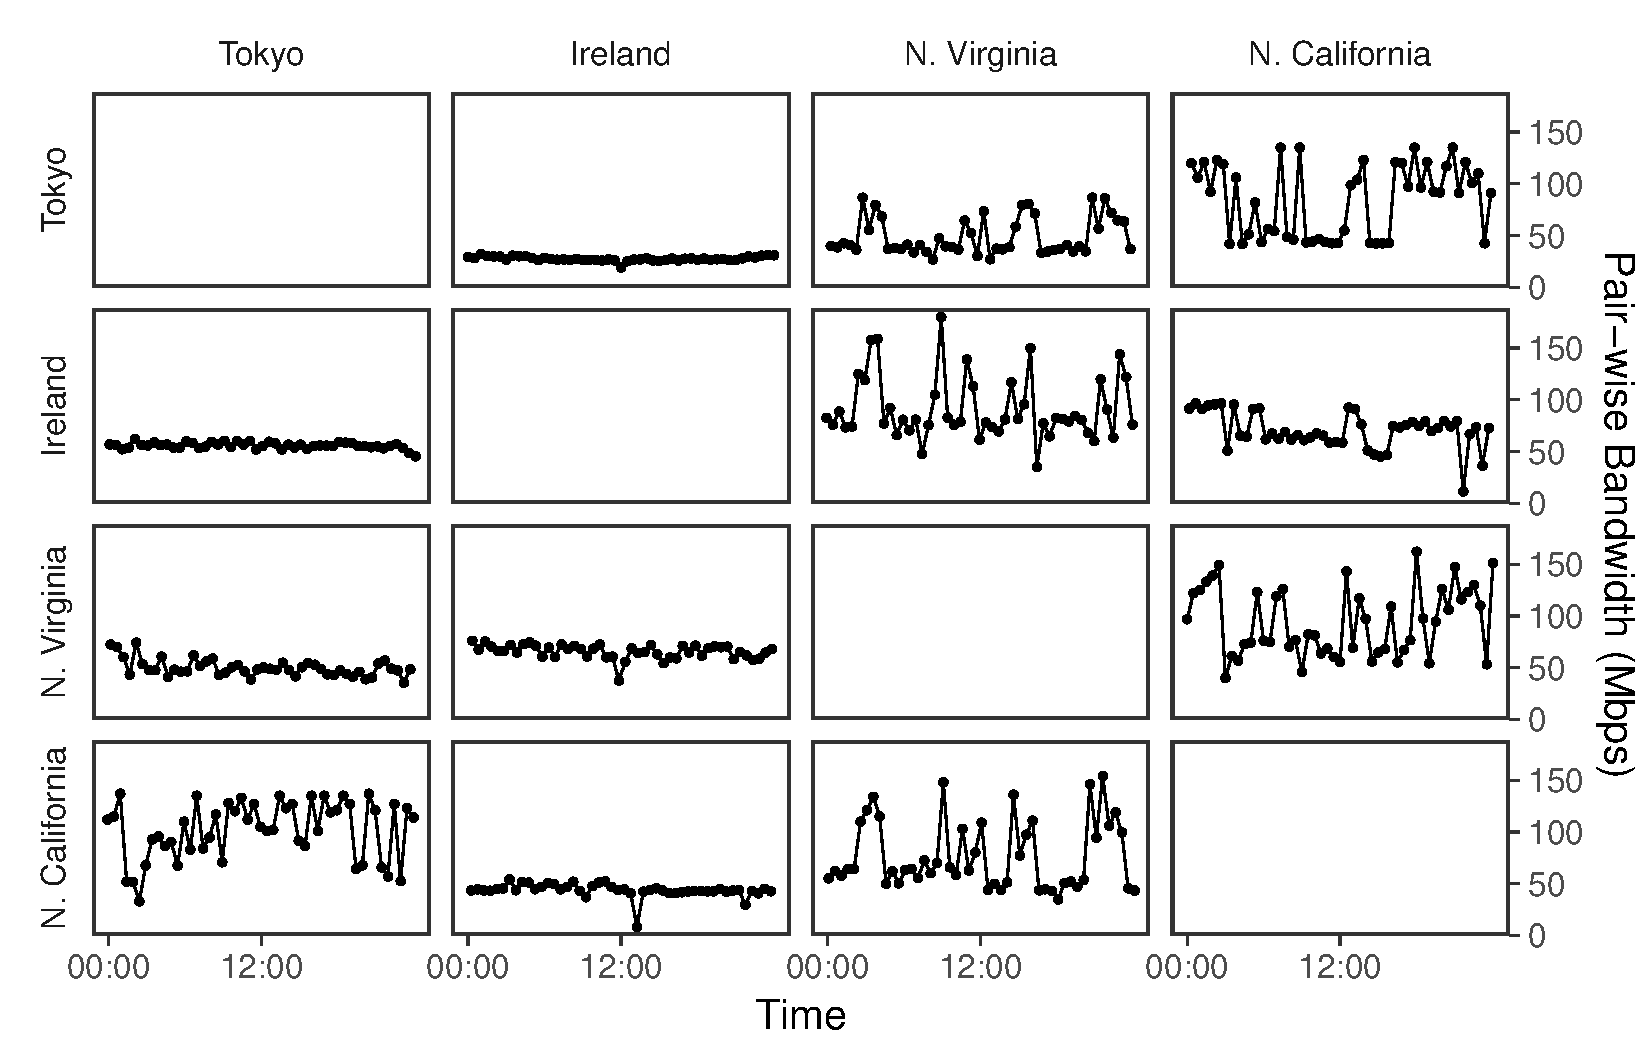
\includegraphics[width=\columnwidth]{figures/aws-bandwidth.pdf}
%   \caption{Pair-wise bandwidth in time series from our day-long measurements.}
%   \label{fig:aws-bandwidth}
% \end{figure}

\section{Additional Information about HLS and JetStream++}
\label{sec:addit-inform-about}

\subsection{HLS Setup}
\label{appendix:hls-setup}

HTTP Live Streaming (HLS)~\cite{pantos2016http} represents a class of HTTP-based
media streaming protocols. Other protocols include Adobe HTTP Dynamic
Streaming~\cite{adobestreaming}, Microsoft Smooth
Streaming~\cite{zambelli2009iis}, and a newer vendor-independent standard
DASH~\cite{michalos2012dynamic, sodagar2011mpeg}. These adaptive streaming
protocols are widely adopted for both video-on-demand (VoD) and live streaming
(such as Periscope).

Our setup (\autoref{fig:hls}) resembles the setup of popular live streaming
services~\cite{wang2016anatomy}. Typical streaming servers set each chunk to be
2-10 seconds~\cite{mao2017neural, sun2016cs2p, wang2016anatomy}. For our low
latency streaming, we configured the chunk segment to be 1 second.

\para{Why HLS/DASH is a poor match for video analytics?} It's hard to achieve
ultra low latency using HLS/DASH: (1) HLS/DASH is pull-based: the client keeps
requesting for new chunks; (2) HLS/DASH uses chunking: shorter chunks enable a
lower latency, but induce a larger number of requests, and the chunk has to be
made ready before the client can start fetching. There are proposals to reduce
the latency, such as server push~\cite{wei2014low}, but they are still work in
progress. For some applications, the accuracy can also be poor if these videos
are limited to tuning resolution and encoding quality only, as demonstrated by
in our PD evaluation.

\begin{figure}[t]
  \centering
  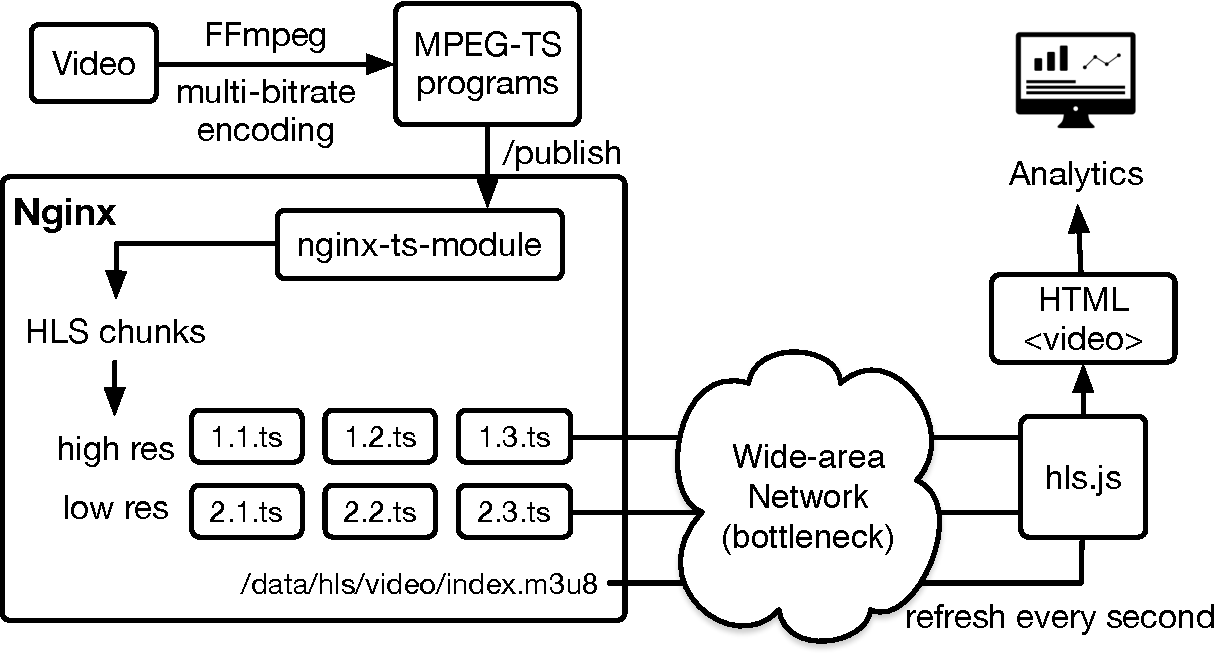
\includegraphics[width=\columnwidth]{figures/hls.pdf}
  \caption{HLS setup: (1)~FFmpeg encodes video with multiple bitrates and groups
    them into MPEG-TS programs;
    (2)~\texttt{nginx-ts-module}~\cite{nginx-ts-module} generates HLS chunks on
    the fly and stores them for nginx serving; (3)~the client (using
    \texttt{hls.js}~\cite{hls.js}) periodically fetches the latest index file
    (\texttt{index.m3u8}) and then downloads the right chunk according to
    network conditions.}
  \label{fig:hls}
\end{figure}

\subsection{JetStream++}
\label{appendix:jetstream++}

We modified the open source version of
JetStream\footnote{\url{https://github.com/princeton-sns/jetstream/}, commit
  bf0931b2d74d20fdf891669188feb84c96AF84.} in order to use our profile as its
manual policy. Because JetStream doesn't support simultaneous degradation across
multiple operators, we implemented a simple \texttt{VideoSource} operator that
understands how to change image resolutions, frame rate, and video encoding
quantization. At runtime, \texttt{VideoSource} queries congestion policy manager
and adjusts three dimensions simultaneously. This operator is then exposed to
the Python-implemented control plane. We call this modified version
JetStream++.\footnote{\url{https://github.com/awstream/jetstream-clone/pull/1}}

JetStream's code base is modular and extensible: the modifications include 53
lines for the header file, 171 lines for implementation, 75 lines for unit test,
and 49 lines of python as the application. While extending JetStream with our
profile is not challenging, JetStream++ performs degradation in a single
operator and loses the composability. We could modify JetStream to support
degradation across multiple operators, but that would require substantial
changes to JetStream. Using JetStream++ with our profile, the comparison is
enough to illustrate the difference between \sysname{}'s and JetStream's
runtime.

%%% Local Variables:
%%% mode: latex
%%% TeX-master: "../network"
%%% End:

%% LocalWords: Mbps analytics runtime JetStream OpenCV YOLO pre GStreamer appsrc
%% LocalWords: appsink zerolatency quantization dataset SVM geo topk VideoSource
%% LocalWords: JetStream's composability TK TCP UDP HLS FFmpeg bitrates nginx
%% LocalWords: packetization TPUT topk NodeJS metadata timestamp Mbps Kbps
%% LocalWords: aws PD's TK's hls js VoD awstream tk fdf feb